\documentclass{beamer}
\usetheme{metropolis}
%\setsansfont[BoldFont={Fira Sans SemiBold}]{Fira Sans Book}
%\setsansfont{Fontin}
%\setsansfont{Gillius ADF No2}
%\setsansfont{Phetsarath OT}
\setsansfont{Source Sans Pro}
\setmonofont{Source Code Pro}

\hypersetup{colorlinks=true,
            linkcolor=mRustLightOrange,
            menucolor=mRustLightOrange,
            pagecolor=mRustLightOrange,
            urlcolor=mRustLightOrange}
\usepackage{csquotes}
\usepackage{comment}
\usepackage{xcolor}
\usepackage{minted}
\usepackage{pdfcomment}
\usepackage{mdframed}
\usepackage{wrapfig}

\newmdenv[linecolor=mRustDarkOrange,roundcorner=10pt,linewidth=1pt,font=\ttfamily]{commandline}

\newfontfamily\codefont{Source Code Pro}
\newcommand\code[1]{\,{\color[HTML]{884400}#1}\,}
\newcommand\source[1]{$\rightarrow$ via #1}
\newcommand\nextline{\hfill{\color{mRustLightOrange}\textbackslash}  \\ }

\renewcommand<>{\talknote}[1]{\only#2{\tikz[remember picture,overlay]{\node{\pdfmargincomment[opacity=0]{#1}}}}\note#2{#1}}

\definecolor{errMsg}{HTML}{CC1100}
\definecolor{warnMsg}{HTML}{EE9900}
\definecolor{refMsg}{HTML}{0011CC}

\newcommand\cmdline[1]{
\begin{commandline}
#1
\end{commandline}
}
\newcommand\opt[1]{
  \texttt{#1}
}

\title{Introduction to rust and its memory safety}
\date{\today}
\author{Lukas Prokop}
\institute{for IAIK\vfill\hfill
\includegraphics[height=2cm]{images/rustacean-orig-noshadow.png}}
\begin{document}
\maketitle

%\section{Prologue}

\begin{frame}[fragile]{About me}
  \begin{itemize}
    \item Software developer
    \item PhD student in post-quantum cryptography at IAIK
    \item Speaker at \href{https://www.meetup.com/Graz-Rust-Meetup/}{RustGraz} (\href{https://twitter.com/RustGraz}{twitter @RustGraz}) \\
      \begin{center}
        
\includegraphics[width=.85\textwidth]{images/rustgraz-meetup.png}
      \end{center}
  \end{itemize}
  \talknote{12 talks compressed to 45min. Condense but well-crafted, Q at end}
\end{frame}

\begin{frame}[fragile]{What is rust?}
  \begin{block}{What is rust?}
    \vspace{10pt}
    \begin{columns}[onlytextwidth,T]
      \column{\dimexpr\linewidth-30mm-5mm}
      \begin{itemize}
        \item multi-paradigmatic \\ (imperative, functional)
        \item systems programming language \\ (easy interop with C, no GC)
        \item focus on memory safety and concurrency
        \item uses the LLVM infrastructure
        \item syntax similar to C++
        \item zero-cost abstractions like C++
        \item Modern competitors: Nim, Crystal, D, Zig
      \end{itemize}
      \column{30mm}
      
\includegraphics[width=\textwidth]{images/rust_logo_wikipedia.pdf}
    \end{columns}
  \end{block}
  \vspace{10pt}
  \enquote{Most loved programming language} \\ (Stack Overflow Developer Survey, 2016--2020)
  \talknote{zero-cost: What you don't use, you don't pay for [Stroustrup, 1994]. And further: What you do use, you couldn't hand code any better.}
\end{frame}

\begin{frame}[fragile]{Rust in academia}
  RustBelt\footnote{\url{http://plv.mpi-sws.org/rustbelt/}}: 32 publications, 4 related projects. \\ August 2020: Ralf Jung's PhD dissertation.

  \begin{center}
    
\includegraphics[width=.9\textwidth]{images/rustbelt.png}
  \end{center}
\end{frame}

% SKIP
%\begin{quote}
%  A longstanding question in the design of programming languages is how to balance safety and control.
%  …
%  Unfortunately, none of Rust's safety claims have been formally investigated, and it is not at all clear that they hold.
%\end{quote}

\begin{frame}[standout]
  Tooling
\end{frame}

\begin{frame}[fragile]{Try it! Rust Playground}
  Rust Playground on \href{https://play.rust-lang.org/}{play.rust-lang.org}

  \begin{center}
    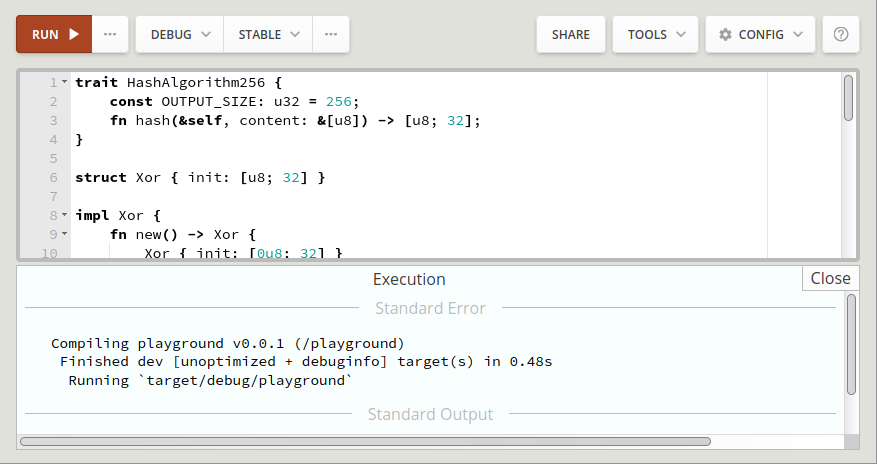
\includegraphics[width=\textwidth]{images/playground.png}
  \end{center}

  Also: rust on \href{https://godbolt.org/}{godbolt.org}
\end{frame}

\begin{frame}[fragile]{Toolchain}
  \cmdline{curl https://sh.rustup.rs -sSf | sh}

  \begin{tabular}{lcc}
    \textbf{First release:} & 1.0 & 2015-05-16 \\
    \textbf{Current release:} & 1.46 & 2020-08-27
  \end{tabular}

  \vspace{17pt}

  Stable rust \href{https://github.com/rust-lang/rust/releases}{releases} \href{https://blog.rust-lang.org/}{every 6 weeks}. Beta and Nightly releases exist. Editions are done every 3 years (2015 1.0 ‘stability’, 2018 1.31 ‘productivity’, 2021 ‘maturity’?)
  \talknote{curl installs rustup which installs cargo and rustc}

  \vspace{10pt}
  \cmdline{rustup install \{stable,beta,nightly\}}
  \cmdline{rustup default \{stable,beta,nightly\}}
\end{frame}

\begin{frame}[fragile]{Rust compiler}
  \vspace{15pt}
  \cmdline{rustup doc --book}
  \cmdline{rustup update}
  \cmdline{rustup self uninstall}
  \vspace{10pt}
  Rust compiler: % featuring \href{https://blog.rust-lang.org/2016/09/08/incremental.html}{incremental compilation} (since rust 1.24):
  %\vspace{-10pt}
  \cmdline{rustc --help}
  \cmdline{rustc --explain E0382}
  %\cmdline{rustc -Z unstable-options \nextline --print target-spec-json PROGRAM.rs}
  \begin{center}
    \textbf{compilation multi-passes:} HIR → MIR → LLVM-IR
  \end{center}
  \talknote{HIR = high-level IR; MIR = mid-level IR \\
  HIR: AST after parsing, macro expansion, and name resolution}
\end{frame}

\begin{frame}[fragile]{Rust compiler}
  \vspace{3pt}
  \cmdline{cargo new [--bin | --lib] NAME}

  %\begin{minted}[highlightlines={1,3,14},highlightcolor=mRustVeryLightOrange,escapeinside=&&,fontsize=\tiny]{text}
  \begin{minted}[escapeinside=~~,fontsize=\tiny]{text}
~\textbf{\$ cargo new --bin iaik}~
     Created binary (application) `iaik` package
~\textbf{\$ tree iaik}~
iaik
├── Cargo.toml
├── .git
│   …
├── .gitignore
└── src
    └── main.rs

10 directories, 18 files

~\textbf{\$ cat iaik/Cargo.toml}~
[package]
name = "iaik"
version = "0.1.0"
authors = ["GIT_COMMITTER_NAME <GIT_COMMITTER_EMAIL>"]
edition = "2018"

# See more keys and their definitions
# at https://doc.rust-lang.org/cargo/reference/manifest.html

[dependencies]
  \end{minted}
  \talknote{bin is default}
  \talknote{“lto = true” to enable link-time optimization}
\end{frame}

\begin{frame}[fragile]{Hello World}
  \begin{minted}{rust}
fn main() {
  println!("Hello, world!");
}
  \end{minted}

  \pause
  \vspace{20pt}
  \hrule{}\vspace{-5pt}
  \begin{minted}[escapeinside=~~,fontsize=\scriptsize]{text}
~\textbf{\$ cargo run}~
   ~\color{gray}{\textit{Compiling} iaik v0.1.0 (/tmp/iaik)}~
    ~\color{gray}{\textit{Finished} dev [unoptimized + debuginfo] target(s) in 0.29s}~
     ~\color{gray}{\textit{Running} `target/debug/iaik`}~
Hello, world!
  \end{minted}
  \hrule{}

  \pause
  \vspace{15pt}
  \href{https://crates.io/}{crates.io} is rust's package index \\
  \opt{--release} for \href{https://doc.rust-lang.org/cargo/reference/profiles.html#release}{optimized build} \\
  \opt{--target TRIPLE} to specify architecture

  \pause
  \vspace{10pt}
  \cmdline{rustc -C opt-level=3 src/main.rs}

  \talknote{default is debug mode}
  \talknote{release is opt-level = 3, still no lto, debug false, overflow checks false}
\end{frame}

\begin{frame}[fragile]{Detect common mistakes}
  \cmdline{rustup component add clippy \\ cargo clippy}

  \begin{minted}[escapeinside=~~,fontsize=\scriptsize]{text}
~\color{warnMsg}{warning: redundant field names in struct initialization}~
   ~\color{refMsg}{--> src/main.rs:114:31}~
    |
114 |   ~\textbf{\_ => Err(BadEncoding\{ encoding: encoding \}),}~
    |                         ^^^^^^^^^^^^^^^^^^ 
    |                help: replace it with: `encoding`
    |
  = note: `#[warn(clippy::redundant_field_names)]` on by default
  = help: for further information visit https://rust-lang.github.io/…
  \end{minted}
\end{frame}

\begin{frame}[fragile]{Normalized code formatting}
  \cmdline{rustup component add rustfmt \\ cargo fmt}

  \begin{minted}[escapeinside=~~,breaklines=true,breakanywhere=true,fontsize=\scriptsize]{text}
~\textbf{% grep -C1 "dst.clone()" main.rs }~
    let dst_encoding = lookup_encoding(
        dst.clone()
    )?;
~\textbf{% cargo fmt --message-format json}~
[{"name":"/home/meisterluk/dev/rust/encconv/src/main.rs","mismatches":[{"original_begin_line":120,"original_end_line":122,"expected_begin_line":120,"expected_end_line":120,"original":"    let dst_encoding = lookup_encoding(\n    dst.clone()\n    )?;","expected":"    let dst_encoding = lookup_encoding(dst.clone())?;"}]}]
  \end{minted}%
  \talknote{like gofmt for golang or black for python}%
  \talknote{slides don't follow coding style due to compactness}%
%
  Also \href{https://github.com/rust-lang/rls}{Rust Language Server}:
  \cmdline{rustup component add rls rust-src \nextline rust-analysis}
  \talknote{rls: goto defs, symbol search, reformatting, code completion, renaming, refactorings}
\end{frame}

\begin{frame}[fragile]{More tools}
  % SKIP \cmdline{cargo run --example EXAMPLE -- arg1 arg2 …}%
  \talknote{example: examples/ folder and NAME.rs contains main, for libs}%
  \vspace{-10pt}
  \cmdline{cargo doc}\vspace{-10pt}
  \begin{center}
    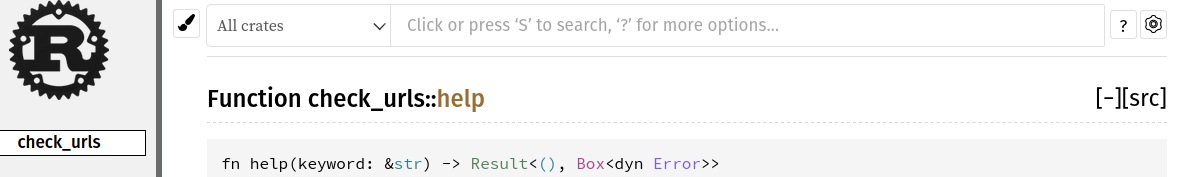
\includegraphics[width=\textwidth]{images/doc-screenshot.png}
  \end{center}
  \talknote{doc gen, and also for its deps, 3 / for doc and Markdown, 2 / for internal comments}%
  \vspace{-20pt}
  \cmdline{cargo test}\vspace{-10pt}
  \begin{center}
    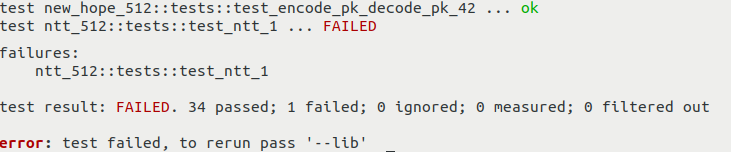
\includegraphics[width=\textwidth]{images/test-screenshot.png}
  \end{center}
  \cmdline{cargo bench}\vspace{-10pt}\talknote{bench attribute is unstable, use 3rd-party-lib criterion}%
\end{frame}

\begin{frame}[standout]
  Syntax and semantics
\end{frame}

\begin{frame}[fragile]{String formatting}
  \begin{minted}[fontsize=\scriptsize]{rust}
fn main() {
  println!("{:09b}=000101010 {:>10}=      IAIK", 42, "IAIK");
  println!("{num:06b}=001010 {who}=rustaceans",
           who = "rustaceans", num = 10);
  let variable = 99;
  println!("{} Luftballoons", variable);
  let l: u64 = 0;
  print!("{}\n", format!("{:04x}", l));
}
  \end{minted}
  \talknote{rust source code: UTF-8 by default}
  \talknote{C\# inspired formatting syntax, we have semicolons}
\end{frame}

\begin{frame}[fragile]{Immutability by default}
  \begin{minted}{rust}
let a: u32 = 0;
a += 1;
  \end{minted}

  \vspace{10pt}
  \hrule{}\vspace{-5pt}
  \begin{minted}[escapeinside=~~,fontsize=\scriptsize]{text}
~\color{errMsg}{error[\textbf{E0384}]: cannot assign twice to immutable variable `a`}~
 ~\color{refMsg}{--> src/main.rs:3:5}~
  |
2 |     ~\textbf{let a: u32 = 0;}~
  |         -
  |         |
  |         first assignment to `a`
  |         help: make this binding mutable: `mut a`
3 |     ~\textbf{a += 1;}~
  |     ^^^^^^ cannot assign twice to immutable variable
  \end{minted}
  \talknote{my favorite feature: type suffix}
\end{frame}

\begin{frame}[fragile]{Immutability by default}
  \begin{minted}{rust}
let mut a: u32 = 0;
a += 1;
\end{minted}
\vspace{48pt}

\begin{minted}{rust}
dbg!(&a);
a = dbg!(&a) + 3;
  \end{minted}
  \talknote{mut, dbg returns its value}

  \hrule{}\vspace{-5pt}
  \begin{minted}{text}
[example.rs:4] &a = 1
[example.rs:5] &a = 1
  \end{minted}
  \hrule{}

  %\vspace{10pt}
  % SKIP  See also: \mintinline{rust}{debug_assert}
\end{frame}

\begin{frame}[fragile]{Primitive types}
  \newcommand\showtype[1]{\textbf{\texttt{\color{mRustLightOrange}#1}}\hspace{15pt}}
  \begin{center}
    \showtype{u8} \showtype{u16} \showtype{u32} \showtype{u64} \showtype{u128} \\
    \showtype{i8} \showtype{i16} \showtype{i32} \showtype{i64} \showtype{i128} \\
    \showtype{isize} \showtype{usize} \showtype{f32} \showtype{f64} \\
    \showtype{bool} \showtype{char}
  \end{center}
  → type suffix notation: \mintinline{rust}{42u8} \\
  → data type boundary value: in stdlib, e.g. \mintinline{rust}{std::u32::MAX}
  \begin{minted}{rust}
42   42_000   0xFF   0o777   0b0010_1010
1.   1e6    -4e-4f64  std::f64::INFINITY
std::f64::NAN  1usize   true   false  'c'
  \end{minted}
  → type inference to determine data type \\
  → default integer type is i32
  \talknote{application for 128-bit integer? IPv6 address, MD5 digest}
  \talknote{char is four bytes in size and represents a Unicode Scalar Value}
  \talknote{usize is 8 bytes on a 64bit-machine}
\end{frame}

\begin{frame}[fragile]{Strings}
  \begin{minted}{rust}
 "C escape sequences\n, Unicode scalars\u{0042}"
\end{minted}
  \begin{minted}{rust}
r"skip \backslash interpretation"
\end{minted}
  \begin{minted}{rust}
b"byte array from ASCII chars"
\end{minted}
  \begin{minted}{rust}
"multiline
 string"
\end{minted}
  \begin{minted}{rust}
"eat all \
      leading whitespace"
\end{minted}
  \let\oldfcolorbox=\fcolorbox
  \AtBeginEnvironment{minted}{\renewcommand{\fcolorbox}[4][]{#4}}
  \begin{minted}{rust}
r#"number of balanced hashes
is arbitrary
"#
  \end{minted}
  \AtBeginEnvironment{minted}{\renewcommand\fcolorbox\oldfcolorbox}
  Two types: \mintinline{rust}{&str} and \mintinline{rust}{String}
  \talknote{String: owned, heap allocated, growable, not null terminated}
  \talknote{\&str: shared, data section, not null terminated}
  \talknote{std::ffi::CString: owned, null terminated}
  \talknote{try to use \mintinline{&str} as much as possible}
\end{frame}

% SKIP strings cannot be indexed
% SKIP “PartialEq versus Eq” here

\begin{frame}[fragile]{Integer semantics}
  \begin{itemize}
    \item \texttt{overflow-checks}: true in debug mode, false in release mode
    \item integer types have method \mintinline{rust}{checked_add}, \mintinline{rust}{overflowing_add}, \mintinline{rust}{saturating_add}, and \mintinline{rust}{wrapping_add}
    \item \mintinline{rust}{u16 as u32} for coercion
    \item Logical left shift. Logical right shift on unsigned integer types. Arithmetic shift on signed integer types.
    \item \mintinline{rust}{assert_eq!(-4 % 7, -4);}
  \end{itemize}
\end{frame}

\begin{frame}[fragile]{Composite types: tuples}
  \begin{minted}{rust}
fn create_tuple() -> (u32, u64) {
  (4, 2)
}

fn main() {
  let (a, b) = (4, 2);

  // comparison by equality
  assert_eq!((4, 2), create_tuple());

  let pair = create_tuple();
  // access by tuple.{zero-based index}
  assert_eq!(a, pair.0);
}
  \end{minted}
  \talknote{max arity 12}
\end{frame}

\begin{frame}[fragile]{Composite types: array}
  \begin{minted}[fontsize=\small]{rust}
let all_zero = [0u8; 32];  // type: [u8; 32]
let mut init = [9, 2, 3];  // type: [{integer}; 3]
let initial  = [1u8, 2, 3];// type: [u8; 3]

init[0] = 1;
//init[4] = 1;  // compile or runtime error
assert_eq!(initial, init);
assert_eq!(initial, initial.clone());

let first_5: &[u8] = &all_zero[0..5];
let first_5: &[u8] = &all_zero[ ..5];
let first_6: &[u8] = &all_zero[0..=5];
  \end{minted}
  \begin{description}
    \item[arrays:] \mintinline{rust}{[u8; 32]}, \mintinline{rust}{[f64; 8]}, \dots
    \item[slices:] \mintinline{rust}{[u8]}, \mintinline{rust}{[f64]}, \dots
  \end{description}
\end{frame}

\begin{frame}[fragile]{Composite types: Vector}
  \mintinline{rust}{std::vec::Vec<T>} is part of the standard library.
  \begin{minted}[fontsize=\footnotesize]{rust}
let mut vec: Vec<u8> = Vec::new();
  \end{minted}
  \vspace{131pt}
\end{frame}

\begin{frame}[fragile]{Composite types: Vector}
  \mintinline{rust}{std::vec::Vec<T>} is part of the standard library.
  \begin{minted}[fontsize=\footnotesize]{rust}
let mut vec = vec![];
  \end{minted}
  \vspace{131pt}
\end{frame}

\begin{frame}[fragile]{Composite types: Vector}
  \mintinline{rust}{std::vec::Vec<T>} is part of the standard library.
  \begin{minted}[fontsize=\footnotesize]{rust}
let mut vec = vec![];
vec[0];
// thread 'main' panicked at
// 'index out of bounds: the len is 0 but the index is 0',
  \end{minted}
  \vspace{93pt}
\end{frame}

\begin{frame}[fragile]{Composite types: Vector}
  \mintinline{rust}{std::vec::Vec<T>} is part of the standard library.
  \begin{minted}[fontsize=\footnotesize]{rust}
let mut vec = vec![];
  \end{minted}
  \vspace{131pt}
\end{frame}

\begin{frame}[fragile]{Composite types: Vector}
  \mintinline{rust}{std::vec::Vec<T>} is part of the standard library.
  \begin{minted}[fontsize=\footnotesize]{rust}
let mut vec = vec![];
vec.push(5);
vec.extend(vec![3, 4]);
vec[0] = 7;
\end{minted}
  \pause
  \begin{minted}[fontsize=\footnotesize]{rust}
assert_eq!(vec[0], 7);
assert_eq!(vec.len(), 3);
assert_eq!(vec.pop(), Some(4));
\end{minted}
  \pause
  \begin{minted}[fontsize=\footnotesize]{rust}
vec.sort();
vec.sort_unstable();
\end{minted}
\pause
  \begin{minted}[fontsize=\footnotesize]{rust}
let elements: &[u8] = &vec[0..2];
  \end{minted}
\end{frame}

% SKIP iteration and iterator trait's functional methods

% https://stackoverflow.com/questions/41034635/idiomatic-transformations-for-string-str-vecu8-and-u8

% SKIP memory layout of Vec, tuple, slices, String, &str, HashMap, …

\begin{frame}[fragile]{Composite types: struct}
  \begin{minted}[fontsize=\small]{rust}
struct HashAlgorithm {
  state: [u8; 32],
  security_margin: u32,
  names: Vec<String>,
}
  \end{minted}
  \pause
  \begin{minted}[fontsize=\small]{rust}
fn main() {
  let h = HashAlgorithm{
    state: [0u8; 32],
    security_margin: 128,
    names: vec!["SHA-2".to_string(),
                "SHA-256".to_string()],
  };
  println!("aliases → {}", h.names.join(", "))
}
  \end{minted}
  \begin{minted}{text}
Output: aliases → SHA-2, SHA-256
  \end{minted}
\end{frame}

% SKIP unit struct, struct with unnamed fields

\begin{frame}[fragile]{Composite types: struct must be sized}
  \begin{minted}[highlightlines={5},highlightcolor=mRustVeryLightOrange,fontsize=\small]{rust}
struct HashAlgorithm {
    state: [u8; 32],
    security_margin: u32,
    names: Vec<String>,
    input_bytes: [u8],
}
  \end{minted}
  Structs must be sized:
  \begin{minted}[escapeinside=~~,fontsize=\tiny]{text}
~\color{errMsg}{error[\textbf{E0277}]: the size for values of type `[u8]` cannot be known at compilation time}~
  ~\color{refMsg}{--> src/main.rs:12:13}~
   |
12 |       let h = HashAlgorithm{state: internal_state,
   |  _____________^
13 | |                           security_margin, names};
   | |_ doesn't have a size known at compile-time _____^
   |
  \end{minted}
\end{frame}

\begin{frame}[fragile]{Composite types: struct: alignment}
  \begin{minted}{rust}
use std::mem::{size_of, align_of};


struct HashAlgo {
  security_margin: u32, //  4 bytes
  names: Vec<String>,   // 24 bytes
  state: [u8; 9],       //  9 bytes
}

fn main() {
  assert_eq!(size_of::<HashAlgo>(), 40);
  assert_eq!(align_of::<HashAlgo>(), 8);
}
  \end{minted}
  \talknote{align of = ABI-required minimum alignment of a type}
  \talknote{rust alignment is allowed to reorder fields}
  \talknote{turbofish operator}
\end{frame}

\begin{frame}[fragile]{Composite types: struct: alignment}
  \begin{minted}{rust}
use std::mem::{size_of, align_of};

#[repr(C)]
struct HashAlgo {
  security_margin: u32, //  4 bytes
  names: Vec<String>,   // 24 bytes
  state: [u8; 9],       //  9 bytes
}

fn main() {
  assert_eq!(size_of::<HashAlgo>(), 48);
  assert_eq!(align_of::<HashAlgo>(), 8);
}
  \end{minted}
  \talknote{}
\end{frame}

\begin{frame}[fragile]{Composite types: struct}
  \begin{minted}[fontsize=\footnotesize]{rust}
#[derive(Debug)]   // HashAlgo { security_margin: 32,
                   // names: [], state: [0, 0 … ] }
struct HashAlgo {
  security_margin: u32, //  4 bytes
  names: Vec<String>,   // 24 bytes
  state: [u8; 9],       //  9 bytes
}
fn main() {
  let h = HashAlgo{ security_margin: 32,
      names: vec![], state: [0u8; 9] };
  println!("{:?}", h);
}
  \end{minted}
  \mintinline{rust}{derive(Debug)} is an attribute macro implementing \mintinline{rust}{Debug} automatically. \\
  \mintinline{rust}{{:?}} asks for \emph{Debug} representation. \\
  \mintinline{rust}{{}} asks for \emph{Display} representation.
\end{frame}

% SKIP
% \begin{frame}[fragile]{Limitation: length of represented arrays}
%   \begin{minted}[fontsize=\scriptsize]{text}
% error[E0277]: arrays only have std trait implementations
%               for lengths 0..=32
%  --> src/main.rs:5:3
%   |
% 5 |   state: [u8; 36],      // 36 bytes
%   |   ^^^^^^^^^^^^^^^ the trait `std::array::LengthAtMost32`
%   |                   is not implemented for `[u8; 36]`
%   |
% \end{minted}
%   Solutions:
%   \begin{itemize}
%     \item Make array small enough
%     \item Implement Debug on your own (not with derive)
%   \end{itemize}
% \end{frame}

\begin{frame}[fragile]{Enumerables}
  \begin{minted}[fontsize=\scriptsize]{rust}
type Digest = [u8; 32];   // type alias: one type, 2 names
\end{minted}
  \pause
  \begin{minted}[fontsize=\scriptsize]{rust}
enum Result {             // enumerable
  Okay(Digest),
  Error(String),
}
\end{minted}
  \pause
  \begin{minted}[fontsize=\scriptsize]{rust}
fn generate_digest() -> Result {
  Result::Okay([42u8; 32])
}
\end{minted}
  \pause
  \begin{minted}[fontsize=\scriptsize]{rust}
fn main() {
  match generate_digest() {
    Result::Okay(d) => {
      for byte in d.iter() {
        print!("{:02X}", byte);
      }
      println!("");
    },
    Result::Error(msg) => eprintln!("error: {}", msg),
  }
}
  \end{minted}
  \talknote{type alias does not introduce new type, two names for 1 type}
  \talknote{internally a discriminator distinguishes enum cases}
  \talknote{match introduces pattern matching, super-powerful!}
  \talknote{eprintln is stderr equivalent of println}
  \talknote{struct and enum together allow to implement Algebraic data types}
\end{frame}

% \begin{frame}[fragile]{Enumerables}
%   \begin{minted}[fontsize=\scriptsize]{rust}
% type Digest = [u8; 32];   // type alias: one type, 2 names

% enum Result {
%     Okay(Digest),
%     Error(String),
% }

% fn generate_digest() -> Result {
%     Result::Error("IV needs to be set".to_string())
% }

% fn main() {
%     match generate_digest() {
%         Result::Okay(d) => {
%             for byte in d.iter() {
%                 print!("{:02X}", byte);
%             }
%             println!("");
%         },
%         Result::Error(msg) => eprintln!("error: {}", msg),
%     }
% }
%   \end{minted}
% \end{frame}

\begin{frame}[fragile]{Error handling in rust}
  \mintinline{rust}{std::result::Result<T, E>}
  \begin{itemize}
    \item \mintinline{rust}{Ok(T)}
    \item \mintinline{rust}{Err(E)}
  \end{itemize}
  No exceptions, no error codes.

  \pause
  \mintinline{rust}{std::option::Option<T>}
  \begin{itemize}
    \item \mintinline{rust}{None}
    \item \mintinline{rust}{Some(T)}
  \end{itemize}

  \pause
  \begin{minted}{rust}
let result = Some(value);
result.unwrap();  // return Some value or panic
result.unwrap_or(default_value);  // … or default
\end{minted}
  \talknote{e.g. Option is returned by Vec.get}
\end{frame}

\begin{frame}[fragile]{Question mark operator}
  The question mark operator exits early in case of \mintinline{rust}{Err}
  or returns the value otherwise.
  \begin{minted}{rust}
fn compile(src: &str) -> Result<(), Error> {
  let tokens = tokenize(&src)?;
  let ast = parse(&tokens)?;
  // …
  Ok(())
}
  \end{minted}
  Return type of function must be a corresponding \mintinline{rust}{Result}.
  \talknote{distinctive operator}
  \talknote{inspired by safe navigation operator}
\end{frame}

\begin{frame}[fragile]{Question mark operator}
  It is can be rewritten with a match expression:
  \begin{minted}{rust}
fn compile(src: &str) -> Result<(), Error> {
  let tokens = match tokenize(&src) {
    Err(E) => return Err(E),
    Ok(ts) => ts,
  };
  let ast = parse(&tokens)?;
  // …
  Ok(())
}
  \end{minted}
\end{frame}

\begin{frame}[fragile]{Control flow}
  \begin{minted}[escapeinside=~~,fontsize=\footnotesize]{rust}
if cond { ~\dots~ } else { ~\dots~ }
if let Some(val) = result { ~\dots~ }

loop { ~\dots~ }
while cond { ~\dots~ }
while let Some(val) = result { ~\dots~ }
for i in 0..1024 { ~\dots~ }
for elem in &vec { ~\dots~ }

let pair = (2, -2);
let kind = match pair {
  (0, 0)                       => "invalid",
  (x @ 1..=5, y) if x + y == 0 => "opposites",
  (x, _)         if x % 2 == 1 => "odd and something",
  _                            => "whatever",
};
println!("{:?} are {}", pair, kind);
  \end{minted}
  \talknote{if: syntax as in Dyalect, Go, Swift, rust}
  \talknote{if let: allows pattern matching}
  \talknote{for: typically with reference}
  \talknote{break and continue; break 'labelled; for nested loops}
  \talknote{match: contrived example, if guards, @ binds, \_ whatever}
  \talknote{everything is an expression: no ternary operator; unit and never data type}
\end{frame}

% SKIP ref keyword

% SKIP source code
% \begin{frame}[fragile]{Beautiful error message example}
%   % TODO example code needed
%   % TODO colors needed
%   \begin{minted}[fontsize=\footnotesize]{text}
% warning: multiple patterns covering the same range
%   --> src/lib/expansion/words/mod.rs:538:36
%     |
% 530 |  b'[' => {
%     |  ---- this range overlaps on `91u8`
% ...
% 538 |  0..=47 | 58..=64 | 91..=94 | 96 | 123..=127 => {
%     |                     ^^^^^^^ overlapping patterns
%   \end{minted}
% \end{frame}

% SKIP can create ranges with floats and test membership (?) but cannot iterate
% SKIP step_by does not accept negative values
% SKIP logical expressions syntax
% SKIP constant globals

\begin{frame}[standout]
  Functions, ownership and borrowing
\end{frame}

\begin{frame}[fragile]{Function syntax}
  % SKIP C++ https://www.bfilipek.com/2020/08/lambda-syntax.html
  % SKIP C++ lambda call: [](){}();
  \begin{minted}[fontsize=\small]{rust}
fn named(name1: T1, name2: T2) -> T_RETURN {}
let unnamed = |name1: T1, name2: T2| -> T_RETURN { };
let short   = |name1    , name2    |             { };
  \end{minted}
  \pause
  Example of anonymous function usage:
  \begin{minted}[fontsize=\small]{rust}
use std::thread;
let handler = thread::spawn(|| {
    println!("Hello World!");
});
handler.join().unwrap();
\end{minted}
  \pause

  Last expression is return value (return keyword only for early exit):
  \begin{minted}[fontsize=\small]{rust}
const fn get_42() -> u32 {
    42
} // const fn = C++ constexpr
\end{minted}%
\talknote{const fn got a lot more powerful in latest release}%
%
\end{frame}

\begin{frame}[fragile]{Function semantics}
  \begin{itemize}
    \item No variadic arguments → slices
    \item Multiple return values → tuples
    \item Functions can be nested
    \item Definitions order in rust does not matter
    \item Blocks \mintinline{rust}{{}} define scopes
    \item \href{https://doc.rust-lang.org/reference/attributes/codegen.html#the-inline-attribute}{inlining} via \mintinline{rust}{#[inline]}, \mintinline{rust}{#[inline(always)]}, or \mintinline{rust}{#[inline(never)]}
  \end{itemize}
  \talknote{blocks can be inserted arbitrarily as in C}
  \talknote{[inline] can be overwritten by compiler (because the instruction cache can become messed up if too many inlines are utilized)}
  \pause
  Memory management notes:
  \begin{itemize}
    \item Stack allocation for local variables
    \item Call by value or call by reference
    \item Arguments and return types must have known size at compilation time
  \end{itemize}
\end{frame}

% SKIP move keyword for anonymous functions

% SKIP rust violates referential transparency: sometimes assignment makes the program compile::
% // replace s with its definition ⇒ crashes
% // this ⇒ compiles.
%
% #![allow(unused)]
% fn main() {
%   let s = String::from(" Mary   had\ta\u{2009}little  \n\t lamb");
%   let mut iter = s.split_whitespace();
%   assert_eq!(Some("Mary"), iter.next());
%   assert_eq!(Some("had"), iter.next());
%   assert_eq!(Some("a"), iter.next());
%   assert_eq!(Some("little"), iter.next());
%   assert_eq!(Some("lamb"), iter.next());

%   assert_eq!(None, iter.next());
% }

\begin{frame}[fragile]{Ownership}
  \begin{itemize}
    % SKIP \item Primitive types are clonable and copyable (\enquote{implement \mintinline{rust}{Copy} and \mintinline{rust}{Clone}})
    \item Each value in Rust has a variable that’s called its \emph{owner}
    \item There can only be one owner at a time
    \item Ownership can \emph{move} from one variable to another
    \item When the owner goes out of scope, the value will be \enquote{dropped}
  \end{itemize}
  \talknote{copy: can be duplicated simply by copying bits}
  \talknote{clone: implements a method to create a clone}
\end{frame}

\begin{frame}[fragile]{Ownership example}
  \begin{minted}[fontsize=\footnotesize]{rust}
#[derive(Debug)]
struct Stats { score: u32 }

fn sub(mut s: Stats) {
  s.score += 1;
}

fn main() {
  let a = Stats { score: 8 };
  sub(a);

}
  \end{minted}%
  \talknote{recognize that a is immutable, s is mutable}
\end{frame}

\begin{frame}[fragile]{Ownership example}
  \begin{minted}[fontsize=\footnotesize]{rust}
#[derive(Debug)]
struct Stats { score: u32 }

fn sub(mut s: Stats) {
  s.score += 1;
}

fn main() {
  let a = Stats { score: 8 };
  sub(a);
  println!("{:?}", a);
}
  \end{minted}
  \talknote{}
\end{frame}

\begin{frame}[fragile]{Ownership example}
  \begin{minted}[escapeinside=~~,fontsize=\footnotesize]{text}
~\color{errMsg}{error[\textbf{E0382}]: borrow of moved value: `a`}~
  ~\color{refMsg}{--> src/main.rs:10:20}~
   |
8  |     ~\textbf{let a = Stats \{ score: 8 \};}~
   |         - move occurs because `a` has type `Stats`,
   |           which does not implement the `Copy` trait
9  |     ~\textbf{sub(a);}~
   |         - value moved here
10 |     ~\textbf{println!("\{\}", a);}~
   |                    ^
   |         value borrowed here after move
  \end{minted}
\end{frame}

\begin{frame}[fragile]{Ownership example}
  \begin{minted}[fontsize=\footnotesize]{rust}
#[derive(Debug)]
struct Stats { score: u32 }

fn sub(mut s: Stats) {
  // owner of Stats instance = `s`
  s.score += 1;
  // `s` goes out of scope → Stats instance is dropped
}

fn main() {
  let a = Stats { score: 8 };
  // owner of Stats instance = `a`
  sub(a); // move Stats instance: `a` → `s`
  println!("{:?}", a); // has been dropped already
}
  \end{minted}
\end{frame}

\begin{frame}[fragile]{Ownership example}
  Solutions:
  \begin{itemize}
    \item Use \mintinline{rust}{#[derive(Debug,Copy,Clone)]}. Then \mintinline{text}{sub} uses copied instance. Results in \mintinline{rust}{Stats { score: 8 }}
    \item Return \mintinline{text}{Stats} instance and assign it again in \mintinline{text}{main}.
    \item Use references (\emph{borrowing} ownership)
  \end{itemize}

  Benefits of ownership for memory safety:
  \begin{itemize}
    \item we can pin-point when a variable is dropped (across threads!)
  \end{itemize}
\end{frame}

\begin{frame}[fragile]{References}
  \begin{minted}{rust}
let mut a = Stats { score: 8 };

let shared_ref = &a;
println!("{:?}", *shared_ref);

let mutable_ref = &mut a;
println!("{:?}", *mutable_ref);
  \end{minted}

  Reference a value with \mintinline{rust}{&}. \\
  Dereference a reference with \mintinline{rust}{*}.
  % SKIP \mintinline{rust}{&5} is a reference to value \mintinline{rust}{5} (assignment required in C).

  \emph{auto-dereferencing:} e.g. \mintinline{rust}{&u32} given, \mintinline{rust}{u32} required? Dereference automatically.
  Best practice: Dereference explicitly.
\end{frame}

\begin{frame}[fragile]{References}
  Rules:
  \begin{itemize}
    \item one or more \emph{shared} references (\mintinline{rust}{&T}) to a resource
    \item exactly one \emph{mutable} reference (\mintinline{rust}{&mut T})
    \item either or, not both! (\enquote{aliasing xor mutation})
  \end{itemize}

  Benefits of reference limitations for memory safety:
  \begin{itemize}
    \item one writer XOR n readers in concurrent context
    \item prevents data races
  \end{itemize}
\end{frame}

% SKIP const *
% SKIP example: “binary operation `+` cannot be applied to type `&mut i32`”

\begin{frame}[fragile]{Ownership example with borrowing}
  \begin{minted}[fontsize=\footnotesize]{rust}
#[derive(Debug)]
struct Stats { score: u32 }

fn sub(s: &mut Stats) {
  s.score += 1;
}

fn main() {
  let mut a = Stats { score: 8 };
  // ownership of `a` is borrowed to `s`
  sub(&mut a);
  // ownership of `s` is returned back to `a`
  println!("{:?}", a);
}
  \end{minted}
\end{frame}

\begin{frame}[fragile]{Lifetimes}
  Basic idea:
  \begin{itemize}
    % SKIP reference to Cyclone programming language inspiring it
    \item How long does the referenced value live?
    \item Where do values live?
      \begin{itemize}
        \item scopes
        \item \mintinline{rust}{'static} (i.e. \enquote{lives as long as the program})
        \item \dots
      \end{itemize}
    \item A lifetime is denoted \mintinline{rust}{'a}, \mintinline{rust}{'b} or \mintinline{rust}{'c}
    \item \emph{Lifetime elision}: compiler has automatic rules which derive lifetimes
    \item In function signatures and struct members, we sometimes need to declare the lifetime explicitly.
  \end{itemize}

  Benefits of lifetimes for memory safety:
  \begin{itemize}
    \item Solves the use-after-free problem
  \end{itemize}
\end{frame}

\begin{frame}[fragile]{Lifetimes example}
  \begin{minted}[fontsize=\footnotesize]{rust}
struct Stats {
  score: &mut u32,
}
  \end{minted}

  \vspace{25pt}
  \dots with lifetimes becomes \dots
  \vspace{25pt}

  \begin{minted}[fontsize=\footnotesize]{rust}
struct Stats<'a> {
  score: &'a mut u32,
}
  \end{minted}
\end{frame}

\begin{frame}[fragile]{Methods}
  \begin{itemize}
    \item methods can be associated with a \mintinline{rust}{struct}
    \item does not depend on \mintinline{rust}{self} → static methods
    \item \mintinline{rust}{let op = Xor::new();} \\
      \mintinline{rust}{op.name()} is syntactic sugar for \mintinline{rust}{Xor::name(op)}
  \end{itemize}

  \vspace{15pt}
  \begin{minted}[fontsize=\footnotesize]{rust}
struct Xor { init: [u8; 32] }

impl Xor {
  fn new() -> Xor {
    Xor { init: [0u8; 32] }
  }
  
  fn name(&self) -> &'static str { "xor" }
}
  \end{minted}
\end{frame}

\begin{frame}[fragile]{Traits}
  \begin{itemize}
    \item Nominal type system, based on Hindley-Milner
    \item traits like contracts, default method implementations possible
    \item trait must be in scope to be used (\mintinline{rust}{use} keyword)
    \item no subtyping, no inheritance, but method overloading
% SKIP
%    \item \textbf{auto traits:}
%      if you implement Trait A, you automatically implement Trait B % not outside stdlib possible?
%    \item \textbf{blanket traits:}
%      conditionally implement a trait for any type that implements another trait
    \item \textbf{marker traits:} no methods to implement, but \mintinline{rust}{impl Trait for Type {}} to declare some property

      e.g. \href{https://doc.rust-lang.org/std/marker/trait.Send.html}{\mintinline{rust}{std::marker::Send}}: Types that can be transferred across thread boundaries.
    \item \textbf{extension traits:}
      Add functionality to primitive/stdlib types
  \end{itemize}

  \vspace{10pt}
  \textbf{Trait coherence:}\vspace{12pt}

  \begin{quote}
    \enquote{%One restriction to note with trait implementations is that 
    … we can implement a trait on a type only if either the trait or the type is local to our crate%. This restriction is part of a property of programs called coherence, and more specifically the orphan rule, so named because the parent type is not present.
    }
  \end{quote}
  \talknote{conceptually a contract, inspired by Haskell typeclasses, Hindley-Milner type system}
\end{frame}

% SKIP extend builtin types with extension traits:
%  trait DoubleExt { fn double(&self) -> Self; }
%  impl DoubleExt for f32 { fn double(&self) -> Self { *self * 2. } }
%  fn main() {
%    let pi = 3.1415926;
%    println!("τ = {}", pi.double());
%    // = 6.283185
%  }

\begin{frame}[fragile]{Traits}
  \begin{minted}[fontsize=\footnotesize]{rust}
trait HashAlgorithm256 {
  const OUTPUT_SIZE: u32 = 256;
  fn hash(&self, content: &[u8]) -> [u8; 32];
}

impl HashAlgorithm256 for Xor {
  fn hash(&self, content: &[u8]) -> [u8; 32] {
    let mut digest = self.init;
    for (i, byte) in content.iter().enumerate() {
      digest[i % 32] ^= byte;
    }
    digest
  }
}
  \end{minted}
\end{frame}

% SKIP Any trait cannot depend on values of other traits.
% SKIP diamond problem exists, but can be disambiguated by removing syntactic sugar

\begin{frame}[fragile]{Generics}
  \begin{itemize}
    \item \mintinline{text}{T} is an abstract type
    \item rust allows to be generic over types (but not values)
    \item implementation by \emph{monomorphization}: \\
          optimized code for each type in executable (like C++ templates)
  \end{itemize}
  \vspace{10pt}
  \begin{minted}[fontsize=\footnotesize]{rust}
fn add<T>(a: T, b: T) -> T
  where T: std::ops::Add<Output = T>
{
  a + b
}

fn main() {
  println!("{}", add(3u8, 5));
  println!("{}", add(3f32, 5.));
}
  \end{minted}
  \talknote{another mechanism: references to traits gives trait objects like Java interfaces}
\end{frame}

% SKIP
% \begin{frame}[fragile]{Trait objects}
%   \mintinline{rust}{dyn Trait} asks for \emph{trait objects} \\
%           like Java interfaces, a runtime object (vtable) is generated containing only method pointers.
%           Requirements:
%           \begin{enumerate}
%             \item All return types must not be Self.
%             \item No generic type parameters.
%           \end{enumerate}
% \end{frame}

% SKIP fn compare(sub1: impl Submission, sub2: impl Submission)  equals  fn compare<T: Submission> (sub1: T, sub2: T) ?
%  trait Smiling { fn smile(&self) -> String; }
%  impl<T: std::fmt::Display> Smiling for T { fn smile(&self) -> String { format!("{} ", self) } }
%  impl<T: std::fmt::Debug> Smiling for T { fn smile(&self) -> String { format!("{} ", self) } }
%  fn main() {
%    println!("{}", "Hello, world!".smile());
%    // ambiguous, does not compile
%  }

% SKIP trait bounds with 2 syntaxi
% SKIP Add, Deref, Drop, Sync, Send, Display, Debug
% SKIP <S as A>::get_x()
% SKIP PhantomData


% SKIP inline assembly example
% #![feature(asm)]
% asm!(assembly template
%   : output operands
%   : input operands
%   : clobbers
%   : options
%   );
% unsafe {
%   // https://stackoverflow.com/a/52050776
%   asm!("leaq (%rip), %rax"
%   : "={rax}"(result)
%   :
%   : "rax"
%   :)
%   }

\begin{frame}[fragile]{unsafe}
  \begin{minted}[fontsize=\footnotesize]{rust}
#[cfg(any(target_arch = "x86", target_arch = "x86_64"))]
fn rdtsc {
    let (mut eax, mut ebx, mut ecx) = (0, 0, 0);
    unsafe {
        asm!("rdtscp",
             out("eax") eax,
             out("ecx") ecx,
             out("edx") edx);
    }
}
  \end{minted}
  \begin{enumerate}
    \item Dereference a raw pointer (\mintinline{rust}{const *})
    \item Call an \mintinline{rust}{unsafe} function or method
    \item Access or modify a mutable static variable
    \item Implement an \mintinline{rust}{unsafe} trait
    \item Access fields of \mintinline{rust}{unions}
  \end{enumerate}
  \talknote{asm!(assembly template, output, input, clobbers, options)}
\end{frame}

\begin{frame}[fragile]{Macros}
  \begin{itemize}
    \item Three kinds of macros
    \begin{enumerate}
      \item function-like macros (\mintinline{rust}{println!("hi")})
      \item derive macros (\mintinline{rust}{derive(Debug)})
      \item attribute-like macros (\mintinline{rust}{cfg(target_arch = "x86")})
    \end{enumerate}
  \end{itemize}
  \begin{minted}[escapeinside=~~,fontsize=\small]{rust}
~\textbf{macro\_rules}~! shake {
  (update $base:ident with $($elem:expr, )*)
    => { $( $base.update($elem); )* };
}
  \end{minted}
  \begin{minted}[escapeinside=~~,fontsize=\small]{text}
~\textbf{Input:}~
  shake!(update h with &data, &[b' '], &data2,);
  \end{minted}
  \begin{minted}[escapeinside=~~,fontsize=\small]{text}
~\textbf{Output:}~
  h.update(&data);
  h.update(&[b' ']);
  h.update(&data2);
  \end{minted}
  \talknote{macros can access and adjust AST}
  \talknote{tokens, not lexical level; whitespace is more limited}
  \talknote{macro hygiene}
\end{frame}

\begin{frame}[fragile]{Stack versus Heap}
  \begin{itemize}
    \item Stack requires \mintinline{rust}{Sized}, opposite is \mintinline{rust}{?Sized}
    \item Heap allocations via special types
    \item e.g. \href{https://doc.rust-lang.org/std/boxed/struct.Box.html}{Box}, \href{https://doc.rust-lang.org/std/rc/struct.Rc.html}{Rc}, \href{https://doc.rust-lang.org/std/sync/struct.Arc.html}{Arc}
  \end{itemize}
  \vspace{15pt}
  \begin{minted}{rust}
fn main() {
  let a = Box::new(5);
  let b = Box::new(6);
  assert_eq!(11, *a + *b);
}
  \end{minted}
\end{frame}

% SKIP? pub for visibility, mod to create modules
% SKIP “a tool for calling C++ from Rust in a heavily automated, but safe, fashion” by Google https://github.com/google/autocxx
% SKIP associated types

% SKIP file operations work with a “Path” as well as a string

\begin{frame}[standout]
  rust is awesome
\end{frame}


\begin{frame}[fragile]{Type inference example}
  Assume \mintinline{rust}{fn store(toml: TomlTree)}.
  \begin{minted}[fontsize=\small]{rust}
let input: &str = r#"[package]\nkey = "value" "#;
match input.parse() {
  Ok(toml) => store(toml),
  Err(error) => panic!("failed to parse TOML"),
};
  \end{minted}

  Implementation of \href{https://doc.rust-lang.org/std/primitive.str.html#method.parse}{str.parse}:
  \begin{minted}[fontsize=\small]{rust}
pub fn parse<F: FromStr>(&self)
    -> Result<F, <F as FromStr>::Err>
{
    FromStr::from_str(self)
}
\end{minted}
\end{frame}

\begin{frame}[fragile]{WebAssembly}
  %\cmdline{rustup target add riscv32imac-unknown-none-elf}
  \cmdline{rustup target add wasm32-unknown-unknown}
  \begin{minted}[fontsize=\scriptsize]{ini}
[dependencies]          # in Cargo.toml
wasm-bindgen = "0.2"
  \end{minted}
  \begin{minted}[fontsize=\scriptsize]{rust}
#[wasm_bindgen]         // in lib.rs
pub fn add(a: i32, b: i32) -> i32 { a + b }
  \end{minted}
  \cmdline{wasm-pack build --target web}
  \begin{minted}[fontsize=\scriptsize]{javascript}
const wasm = await init("./pkg/webassembly_example_bg.wasm");
const sum = wasm.add(20, 22);
document.body.textContent = `computed in WASM: ${sum}`;
  \end{minted}
  \begin{center}
    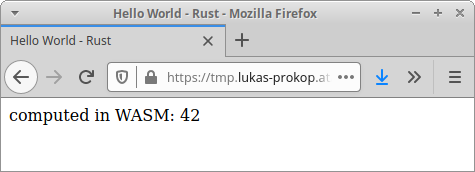
\includegraphics[width=.6\textwidth]{images/wasm.png} \\
    via \href{https://wasmbyexample.dev/examples/hello-world/hello-world.rust.en-us.html}{wasmbyexample.dev}
  \end{center}
\end{frame}

\begin{frame}[fragile]{Critical parts}
  \begin{itemize}
    \item Long compilation times
      \begin{itemize}
        \item compare with golang
        \item see also \href{https://perf.rust-lang.org/}{perf.rust-lang.org}
      \end{itemize}
    \item Multi-pass compiler
      \begin{enumerate}
        \item fix lexical errors
        \item fix types
        \item fix borrows
        \item fix lifetimes
        \item \dots
      \end{enumerate}
    \item \href{https://www.reddit.com/r/rust/comments/33jv62/vecrcrefcellboxtrait_is_there_a_better_way/}{\enquote{\mintinline{rust}{Vec<Rc<RefCell<Box<Trait>>>>}? \\ Is there a better way?}}
  \end{itemize}
\end{frame}

\begin{frame}[fragile]{Resources}
  Official documentation:
  \begin{itemize}
    \item \href{https://doc.rust-lang.org/stable/book/}{Rust book}
    \item \href{https://doc.rust-lang.org/stable/rust-by-example/}{Rust by example}
    \item Rust website: \href{https://www.rust-lang.org/learn}{learn page}
    % SKIP \item \href{https://doc.rust-lang.org/nomicon/}{Nomicon: internals of rust}
  \end{itemize}
  Event-based:
  \begin{itemize}
    \item \href{https://2020.rustfest.eu/}{RustFest conference} (talks on youtube)
    \item \href{https://www.meetup.com/Graz-Rust-Meetup/}{RustGraz} local meetup
  \end{itemize}
  Book: \href{https://www.manning.com/books/rust-in-action}{Rust in Action}
\end{frame}

\begin{frame}
  \begin{center}
    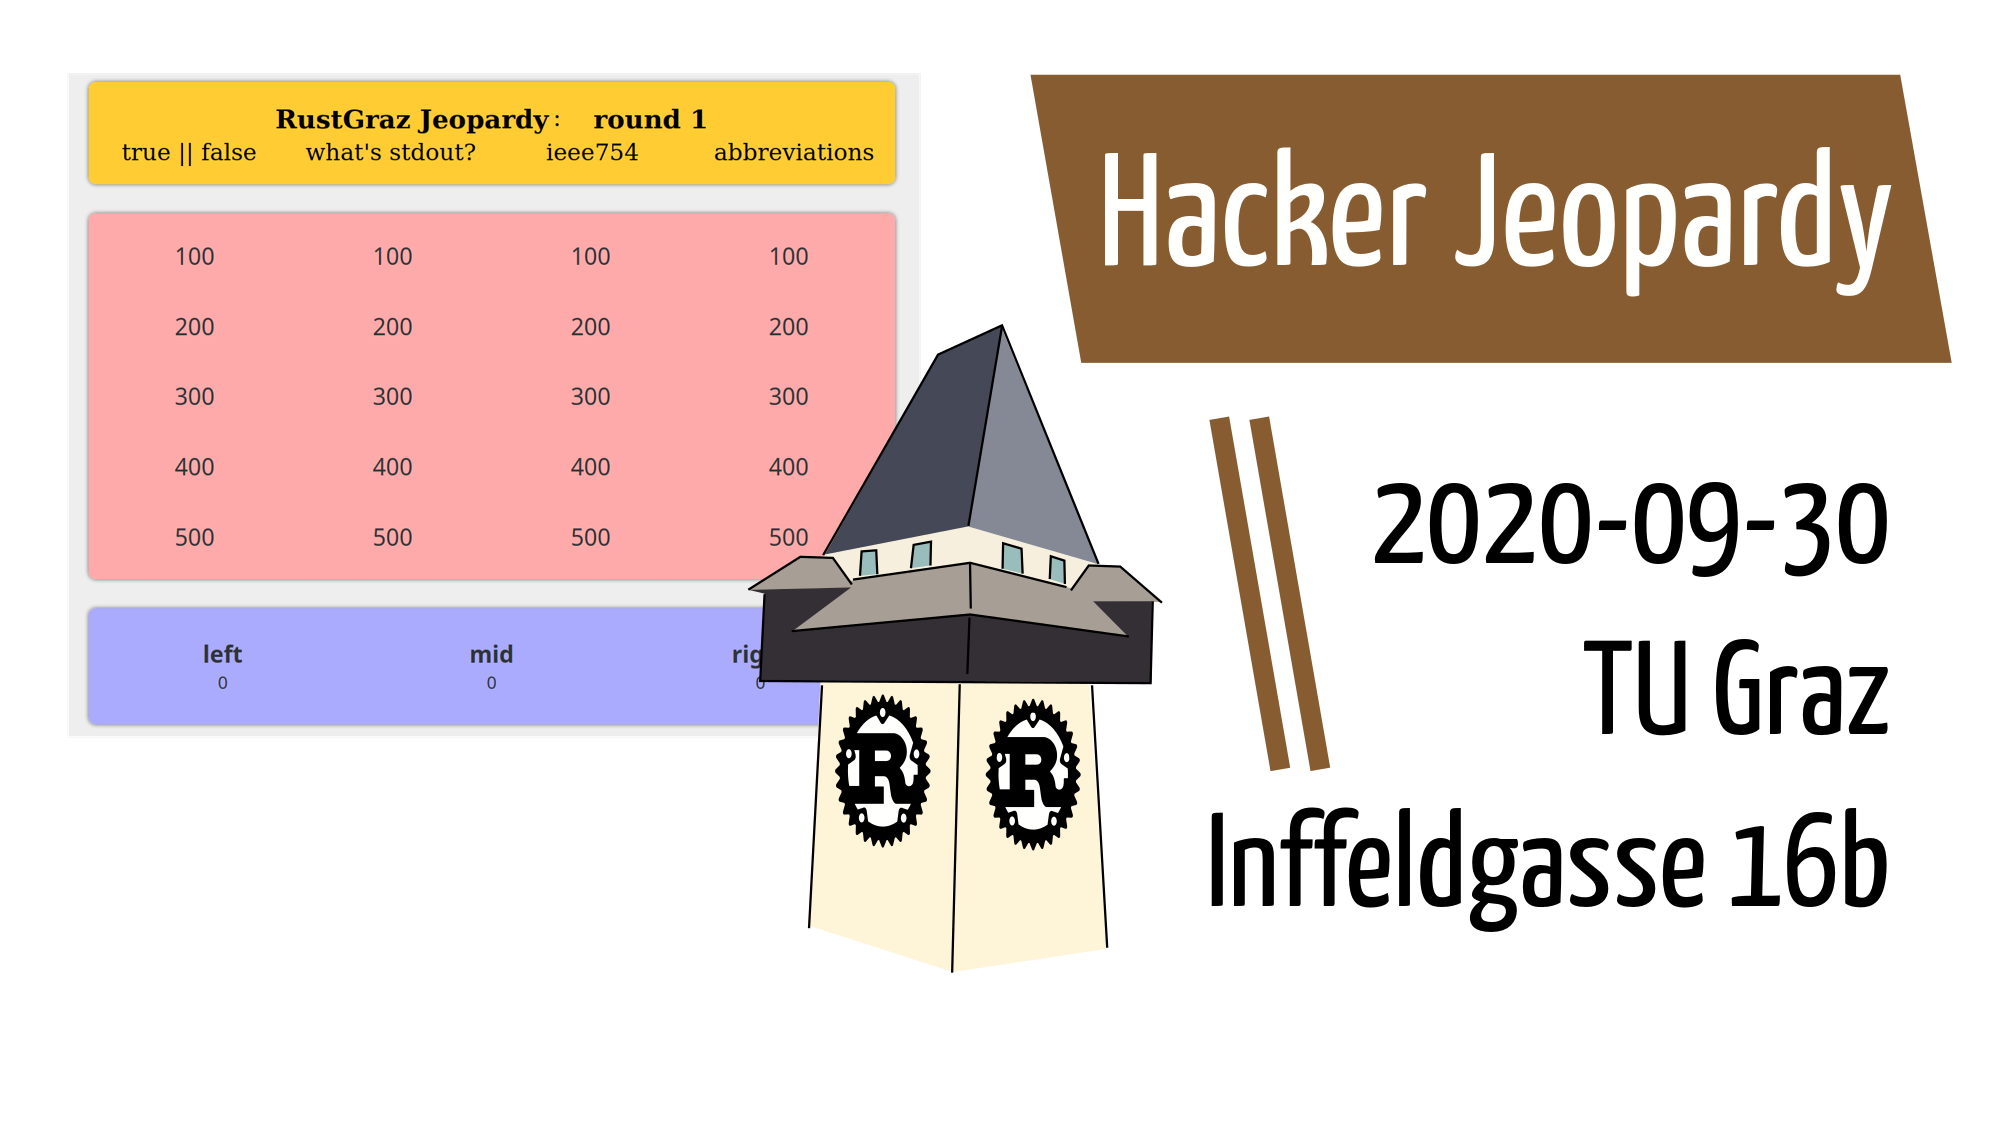
\includegraphics[width=\textwidth]{images/2020-09-talk.png}
  \end{center}
\end{frame}

% TODO github examples link

\begin{frame}[standout]
  Thank you! Q/A? \\[30pt]

  
\includegraphics[width=100pt]{images/rustacean-flat-happy.png}
\end{frame}

\begin{frame}[fragile]{Concurrency}
  \begin{itemize}
    \item SIMD, atomic ops, Mutex/CondVar, Once, RwLock, Barrier
    \item crossbeam-channel
    \item OS threads
    \item async \& await since rust 1.39 requires executor/reactor/waiter like tokio/smol/async-std uses Futures
    \item shared memory
  \end{itemize}
\end{frame}

\begin{frame}[fragile]{Concurrency}
  Are we \dots yet?
  \begin{itemize}
    \item \href{https://www.areweguiyet.com/}{GUI}
    \item \href{https://www.arewelearningyet.com/}{(Machine) learning}
    \item \href{https://www.arewewebyet.org/}{Web}
    \item \href{https://arewegameyet.rs/}{game}
    \item \href{https://areweaudioyet.com/}{audio}
  \end{itemize}
  via \href{https://wiki.mozilla.org/Areweyet}{Mozilla: Areweyet}
\end{frame}

\end{document}
